\documentclass[a4paper]{report}
\usepackage{amsmath}
\usepackage{amssymb}
\usepackage{caption}
\usepackage[mathscr]{eucal}
\usepackage{graphicx}
\usepackage{hyperref}
\usepackage{pgfplots}
\usepackage{subfigure}
\usepackage{xcolor}

% Uguaglianze/relazioni
\newcommand\aceq{\stackrel{\mathclap{\normalfont\mbox{ac}}}{\;=\;}}
\newcommand{\indep}{\mathrel{\text{\scalebox{1.07}{$\perp\mkern-10mu\perp$}}}}
\newcommand{\iidsim}{\stackrel{\text{iid}}{\sim}}
\newcommand{\indsim}{\stackrel{\indep}{\sim}}
\newcommand{\notindep}{\centernot{\indep}}

% Vari
\newcommand{\Ind}{\mathds{1}} % indicatrice
\newcommand{\im}{\operatorname{im}}
\newcommand{\markov}{\operatorname{Markov}}
\newcommand{\uu}[1]{\underline{#1}} % per i vettori
\newcommand{\IS}{È }
\renewcommand{\theta}{\vartheta} % è molto più bella

% Lettere fighe/corsive
\newcommand{\Ac}{\mathcal A}
\newcommand{\Bc}{\mathcal B}
\newcommand{\Cc}{\mathcal C}
\newcommand{\Dc}{\mathcal D}
\newcommand{\Ec}{\mathcal E}
\newcommand{\Fc}{\mathcal F}
\newcommand{\Gc}{\mathcal G}
\newcommand{\Hc}{\mathcal H}
\newcommand{\Ic}{\mathcal I}
\newcommand{\Jc}{\mathcal J}
\newcommand{\Kc}{\mathcal K}
\newcommand{\Lc}{\mathcal L}
\newcommand{\Mc}{\mathcal M}
\newcommand{\mm}{\mathscr m} %per la misura di Lebesgue
\newcommand{\Nc}{\mathcal N}
\newcommand{\Oc}{\mathcal O}
\newcommand{\Pc}{\mathcal P}
\newcommand{\Qc}{\mathcal Q}
\newcommand{\Rc}{\mathcal R}
\newcommand{\Sc}{\mathcal S}
\newcommand{\Tc}{\mathcal T}
\newcommand{\Uc}{\mathcal U}
\newcommand{\Vc}{\mathcal V}
\newcommand{\Wc}{\mathcal W}
\newcommand{\Xc}{\mathcal X}
\newcommand{\Yc}{\mathcal Y}
\newcommand{\Zc}{\mathcal Z}

% Doppia barra
\renewcommand{\AA}{\mathbb A}
\newcommand{\BB}{\mathbb B}
\newcommand{\CC}{\mathbb C}
\newcommand{\DD}{\mathbb D}
\newcommand{\EE}{\mathbb E}
\newcommand{\FF}{\mathbb F}
\newcommand{\GG}{\mathbb G}
\newcommand{\HH}{\mathbb H}
\newcommand{\II}{\mathbb I}
\newcommand{\JJ}{\mathbb J}
\newcommand{\KK}{\mathbb K}
\newcommand{\LL}{\mathbb L}
\newcommand{\MM}{\mathbb M}
\newcommand{\NN}{\mathbb N}
\newcommand{\OO}{\mathbb O}
\newcommand{\PP}{\mathbb P}
\newcommand{\QQ}{\mathbb Q}
\newcommand{\RR}{\mathbb R}
\renewcommand{\SS}{\mathbb S}
\newcommand{\TT}{\mathbb T}
\newcommand{\UU}{\mathbb U}
\newcommand{\VV}{\mathbb V}
\newcommand{\WW}{\mathbb W}
\newcommand{\XX}{\mathbb X}
\newcommand{\YY}{\mathbb Y}
\newcommand{\ZZ}{\mathbb Z}

% d nell'integrale
\newcommand{\de}{\mathrm d}
\newcommand{\dx}{\de x}
\newcommand{\dy}{\de y}
\newcommand{\dP}{\de P}
\newcommand{\dPP}{\de \PP}


\title{\texttt{bnplib}: A Nonparametric C++ Library}

\author{
Bruno Guindani \\
Elena Zazzetti \\
\\
Professor: Alessandra Guglielmi \\
Advisor: Mario Beraha \\
\\
\\
Politecnico di Milano \\
\\
}

\date{
February 19, 2020
\\[250pt]
{\color{gray} {\url{https://github.com/poliprojects/BNPlib}}}}

\begin{document}

\maketitle

\begin{abstract}
We present a C++ library that exploits a Bayesian nonparametric setting in order to conduct monodimensional data analysis.
In such a setting, our main goals are density estimation and clustering analysis.
Several algorithms are available that make use of Gibbs sampling, building a Markov chain that reaches convergence at a reasonably fast pace.
In particular, we focused on implementing some algorithms introduced by Neal in 2000.
After running one of these algorithms, density and cluster estimation can then be conducted by using the provided auxiliary tools.
In this report, after an overview of the underlying Bayesian model and a roundup of the algorithms' state of the art, we delve into the details of our implementation and then present an example of data analysis, whilst providing the theoretical background for our estimates.
\end{abstract}
\clearpage

\tableofcontents

\part{Algorithms}

\chapter{Introduction}
This report presents the development of a C++ library containing Markov chain sampling algorithms for two major goals: estimation of the density and clustering analysis of a given set of data points.
In a Bayesian nonparametric setting, we focused on the Dirichlet process, one of the most widely used priors due to its flexibility and computational ease, and its extensions.
Hereafter, we will assume that the underlying model for the given data points is a Dirichlet process mixture model, which is an enhancement of the simpler Dirichlet model.
We shall now briefly describe these models and their relevant properties.
(For a more detailed discussion of the nonparametric models, as well as references for all theoretical details included in this section, see \cite{book} chapter 1 and 2.)

\section{Dirichlet process model}
Let $M>0$, and let $G_0$ be a probability measure defined on the state space $S$.
A Dirichlet process with parameters $M$ and $G_0$, noted as $DP(M,G_0)$, is a random probability measure $G$ defined on $S$ which assigns probability $G(B)$ to every set $B$ such that for each finite partition ${B_1,\dots,B_k}$ of $S$, the joint distribution of the  vector $(G(B_1),\dots,G(B_k))$ is the Dirichlet distribution with parameters
\begin{align*}
(MG_0(B_1),\dots,MG_0(B_k)).
\end{align*}
The parameter $M$ is called the precision or total mass parameter, $G_0$ is the centering measure, and the product $MG_0$ is the base measure of the DP. \\
Having observed the independent and identically distributed sample $\{y_1,\dots,y_n\}$ \\*
$\subseteq \RR$, the basic DP model takes the following form:
\begin{equation}
	\begin{aligned}
	y_i | G &\iidsim G, \quad i=1,\dots,n \\
	G &\sim DP(MG_0)
	\end{aligned}
\end{equation}
A key property is that the DP is conjugate with respect to iid sampling, so that the posterior base distribution is a weighted average of the prior base distribution $G_0$ and the empirical distribution of the data, with the weights controlled by $M$:
\begin{align}
	G | y_1,\dots,y_n \sim DP\left(M G_0 + \sum_{i=1}^n \delta_{y_i}\right).
\end{align}
Moreover, the marginal distribution for the data will be the product of the sequence of increasing conditionals:
\begin{align*}
	p(y_1,\dots,y_n)= p(y_1)\prod\limits_{i=2}^{n} p(y_i|y_1,\dots,y_{i-1}),
\end{align*}
with $y_1 \sim G_0$ and the conditional for $i=2,3,\dots$ being the following:
\begin{align*}
	p(y_i|y_1,\dots,y_{i-1})= \frac{1}{M+i-1}\sum_{h=1}^{n-1} \delta_{y_h}(y_i) +\frac{M}{M+i-1} G_0(y_i).
\end{align*}
Another important property is the discrete nature of the random probability measure $G$.
Because of this, we can always write $G$ as a weighted sum of point masses.
A useful consequence of this property is its stick-breaking representation, i.e. $G$ can be written as:
\begin{align*}
	G(\cdot) = \sum_{k=1}^{+\infty} w_k \delta_{m_k} (\cdot),
\end{align*}
with $m_k \iidsim G_0$ for $k\in\mathbb{N}$ and the random weights constructed as $w_k =v_k\prod\limits_{l<k} (1-v_l)$ where $v_k \iidsim Be(1,M)$. \\
In many applications in which we are interested in a continuous density estimation, this discreteness can represent a limitation.
Oftentimes a Dirichlet process mixture (DPM) model is used, where the DP random measure is the mixing measure for the parameters of a parametric continuous kernel function.

\section{Dirichlet process mixture model}
Let $\Theta$ be a finite-dimensional parameter space and $G_0$ a probability measure on $\Theta$.
The Dirichlet process mixture (DPM) model convolves the densities $f(\cdot|\boldsymbol\theta)$ from a parametric family $\Fc = \{f(\cdot|\boldsymbol\theta), \boldsymbol\theta \in \Theta \}$ using the DP as mixture weights.
The obtained model has the following form:
\begin{equation}
	\begin{aligned}\label{dpm-1}
	y_i | G &\iidsim f_G(\cdot) = \int_\Theta f(\cdot|\boldsymbol\theta) \, G(\de\boldsymbol\theta), \quad i=1,\dots,n \\
	G &\sim DP(M G_0)
	\end{aligned}
\end{equation}
An equivalent hierarchical model is:
\begin{equation}
	\begin{aligned}\label{dpm-2}
	y_i | \boldsymbol\theta_i &\indsim f(\cdot|\boldsymbol\theta_i), \quad i=1,\dots,n \\
	\boldsymbol\theta_i | G &\iidsim G, \quad i=1,\dots,n \\ 
	G &\sim DP(M G_0)
	\end{aligned}
\end{equation}
where the \emph{latent variables} $\boldsymbol\theta_i$ are introduced, one per unit.
Since $G$ is discrete, we know that two independent draws $\boldsymbol\theta_i$ and $\boldsymbol\theta_j$ from $G$ can be equal with positive probability.
In this way the DPM model induces a probability model on clusters of $\boldsymbol\theta_i$.
An object of interest that derives from this model is the partitioning induced by the clustering. \\%, as well as the density estimation. \\
Considering $n$ data points, each $\boldsymbol\theta_i$ will have one of the $k$ unique values $\boldsymbol\phi_{j}$.
An estimation of the number of the unique values is $M\log(n) \ll n$.
Defining  $\boldsymbol c= (c_1,\dots,c_n)$ the \emph{allocation} parameters to the clusters such that $c_i = j$ if $\boldsymbol\theta_i = \boldsymbol\phi_j$, model (\ref{dpm-2}) can be thought of as the limit as $K \to +\infty$  of a finite mixture model with $K$ components (recall instead that $k$ is the number of unique values):
\begin{equation}
	\begin{aligned}\label{dpm-disc}
		y_{i}|\boldsymbol{\phi}_1,\dots,\boldsymbol{\phi}_k,c_{i} &\indsim f(\cdot|\boldsymbol\phi_{c_{i}}), \quad i=1,\dots,n \\
		c_{i}|\mathit{\mathbf{p}}&\iidsim \sum_{j=1}^K\mathit{p_j} \delta_j(\cdot), \quad i=1,\dots,n \\
		\boldsymbol\phi_{c} & \iidsim G_{0}, \quad c=1,\dots,k \\
		\mathbf{p} &\sim \operatorname{Dir}(M/K,\dots,M/K)
	\end{aligned}
\end{equation}
where $\mathbf{p}=(p_1,\dots,p_K)$ represents the mixing proportions for the clusters and each $\boldsymbol\theta_i$ is characterized by the latent cluster $c_i$ and the corresponding parameters $\boldsymbol\phi_{c_i}$.

\subsection{Normal Normal-InverseGamma model} \label{nnig}
A very common choice for the DPM model (\ref{dpm-1}) is the Normal Normal-InverseGamma (Normal-NIG) model, opting for a Normal kernel and the conjugate Normal-InverseGamma as base measure $G_0$. That is, letting $\boldsymbol\theta=(\mu,\sigma)$, we have:
\begin{equation}
	\begin{aligned}
		f(y|\boldsymbol\theta)&=N(y| \mu ,\sigma^2),  \\
		G_0(\boldsymbol\theta|\mu_0,\lambda_0, \alpha_0, 	\beta_0)
		&=N\left(\mu | \mu_0 ,\frac{\sigma^2} {\lambda_0}\right) \times \text{Inv-Gamma}(\sigma^2|\alpha_0, \beta_0 ).
	\end{aligned}
\end{equation}
Note that in this model we have a full prior for $\sigma^2$ and instead a prior for $\mu$ that is conditioned on the value of $\sigma^2$.
Thanks to conjugacy, the predictive distribution for a new observation $\widetilde{y}$ can be computed analytically, finding a Student's $t$ (see \cite{integral} section 3.5):
\begin{align*}
	p(\widetilde{y}|\mu_0,\lambda_0, \alpha_0, \beta_0) =
	\int_\Theta f(\widetilde{y}|\boldsymbol\theta) \, G_0(\de\boldsymbol\theta) =
	\text{t}_{\widetilde \nu}\left(\widetilde{y}|\widetilde{\mu},\widetilde{\sigma}\right)
\end{align*}
where the following parameters are set:
$$
	\widetilde{\nu}=2 \alpha_0, \quad
	\widetilde{\mu}=\mu_0, \quad
	\widetilde{\sigma}^2= \frac{\beta_0(\lambda_0+1)}{\alpha_0 \lambda_0}
$$
Moreover, the marginal distribution for a given observation has the same expression. \\
The posterior distribution is again a Normal-InverseGamma (see \cite{integral} section 3.3):
\begin{align*}
	p(\boldsymbol\theta|y_1,\dots,y_n,\mu_0,\lambda_0, \alpha_0, \beta_0)=N\left(\mu | \mu_n ,\frac{\sigma^2} {\lambda_0 + n}\right) \times \text{Inv-Gamma}(\sigma^2|\alpha_n, \beta_n )
\end{align*}
with:
$$
\mu_n=\frac{\lambda_0 \mu_0 \bar{y} + n}{\lambda_0 + n}, \quad \alpha_n= \alpha_0 + \frac{n}{2}, \quad \beta_n= \beta_0 + \frac{1}{2}\sum_{i=1}^{n} (y_i-\bar{y})^2 + \frac{\lambda_0 n(\bar{y}-\mu_0)^2}{2(\lambda_0 + n)}.
$$

\chapter{Algorithms} \label{algo}
For the task of density estimation, we investigated several Markov chain methods to sample from the posterior distribution of a DPM model. \\
Starting from the hierarchical model (\ref{dpm-1}), a first direct approach is simply drawing values for each $\boldsymbol\theta_i$ from its conditional distribution, given the data and the other $\boldsymbol\theta_j$.
However, as previously discussed, we have high probability for ties among them which can lead to slow convergence, since the $\boldsymbol\theta_i$ are not updated for more than one observation simultaneously. \\
For this reason, special attention was paid to the three methods we present in this chapter.
They are Gibbs samplers with a similar base structure, sharing the two steps for the sampling of the allocations $\mathbf{c}$ and of the unique values $\boldsymbol\phi_c$.
The set of allocations and unique values at a given iteration constitutes the \emph{state} of that iteration.
As the state is being updated at each iteration, a \emph{chain} is formed and the mean of the state values eventually reaches convergence, as well as the estimate for the data distribution, as we will see in section \ref{dens-estim}.
Moreover, all methods can be extended with additional steps for hierarchical extensions.
For example, we can place priors to hyperparameters of the centering measure $G_0$ or to the total mass $M$.

\section{Neal's Algorithm 2} \label{neal2}
In order to speed up convergence in case of ties, Neal first proposed (see \cite{neal} section 3 as well as \cite{book} chapter 2) a more efficient Gibbs sampling method based on the discrete model (\ref{dpm-disc}), but where the mixing proportions $\textbf{p}$ have been integrated out.
We will refer to this method as Neal's Algorithm 2, or \verb|Neal2| for short.
Before getting to the algorithm, let us start from the discrete model (\ref{dpm-disc}).
Assuming that the current state of Markov chain is composed of $(c_1,\dots,c_n)$  and the unique values $\boldsymbol\phi_c$ for all $c=1,\dots,k$, the Gibbs sampler should first draw a new value $c$ for each $c_i$ according to the following probabilities:
\begin{align}
	\hspace{-25pt}
	\vspace{-12pt}
	\text{If $c=c_j$ for some $j$: }
	\PP(c_{i}=c | \boldsymbol c_{-i}, y_{i},\boldsymbol{\phi}_1,\dots,\boldsymbol{\phi}_k) \propto \frac{n_{-i,c} + M/{K}}{n-1+M} f(y_{i}|\boldsymbol\phi_{c}) 
\end{align}
where $\boldsymbol c_{-i}$ is $\boldsymbol c$ minus the $i$-th component, and $n_{-i,c}$ is the number of $c_j$ equal to $c$ excluding $c_i$.
The transition to the infinite case, that is, to the reference DPM model (\ref{dpm-2}), is handled by taking the limit as $K$ goes to infinity in the conditional distribution of $c_i$, which becomes as follows:
\begin{equation}
	\begin{aligned} \label{probasneal2}
	\hspace{-25pt}
	\vspace{-12pt}
	\text{If $c=c_j$ for some $j$: }
	\PP(c_{i}=c | \boldsymbol c_{-i}, y_{i}, \boldsymbol{\phi}_1,\dots,\boldsymbol{\phi}_k) &\propto \frac{n_{-i,c} }{n-1+M} f(y_{i}|\boldsymbol\phi_{c}) \\
	\PP(c_{i}\neq c_{j} \text{ for all } j | \boldsymbol c_{-i}, y_{i}, \boldsymbol{\phi}_1,\dots,\boldsymbol{\phi}_k) &\propto \frac{M }{n-1+M} \int_{\Theta} f(y_{i}|\boldsymbol\theta) \, G_0(\de\boldsymbol\theta)
	\end{aligned}
\end{equation}
and considering only the $\boldsymbol\phi_c$ associated with some observation, keeping the sampling finite and thus computationally feasible.
The former expression is proportional to the cardinality of that cluster (excluding the $i$-th observation), while the latter is instead proportional to the total mass $M$ and represents the probability of creating a new cluster.
Moreover, the integral $m(y_i) = \int_{\Theta} f(y_{i}|\boldsymbol\theta) \, G_0(\de\boldsymbol\theta)$ represents the \emph{marginal distribution} of the data points evaluated in $y_i$. \\
Let us now introduce the actual \verb|Neal2| algorithm, which works iteratively in two steps, in which we sample $(\boldsymbol{c}_1,\dots,\boldsymbol{c}_n)$ and $(\boldsymbol{\phi}_1,\dots,\boldsymbol{\phi}_k)$, respectively.
First, for each observation $i$, $c_i$ is updated according to the conditional probabilities (\ref{probasneal2}).
It can be set either to one of the other components currently associated with some observation, or to a new mixture component.
If the new value of $c_i$ is different from all the other $c_j$, a value for $\boldsymbol\phi_{c_i}$ is created by drawing it from the posterior distribution $H_i$, given the prior $G_0$ and the single observation $y_i$; this means that in this case, a new cluster has been created. \\
Then, for all clusters, the sampling of their unique value $\boldsymbol\phi_c$ is conducted by considering their posterior distribution given the prior $G_0$ and all observations belonging to that cluster.
The probability of setting $c_i$ to a new component involves the computation of the marginal, which is difficult to compute in the non-conjugate case, as well as the sampling from the posterior $H_i$.
For this reason, the algorithm is only used under conjugacy and hence it is possible to exactly compute the integral.

\section{Neal's Algorithm 8} \label{neal8}
To handle non-conjugate priors, Neal proposed (see \cite{neal} section 6 and \cite{book} chapter 2) a second Markov chain sampling procedure, the \verb|Neal8| algorithm, where the state is extended by the addition of $m$ auxiliary parameters.
This technique allows to update the $c_i$ while avoiding the integration with respect to $G_0$ for the computation of the marginal. \\
In this case the sampling probabilities for the $c_i$ given all other $c_j$ are:
\begin{equation}
	\begin{aligned}
		\hspace{-25pt}
		\vspace{-12pt}
		\text{If $c=c_j$ for some $j$: } \PP(c_i=c | \boldsymbol c_{-i}) &= \frac{n_{-i,c}}{n-1+M}   \\
		\PP(c_{i}\neq c_{j} \text{ for all } j) &=\frac{M }{n-1+M}
	\end{aligned}	
\end{equation}
where the latter probability of creating a new cluster is evenly split among the $m$ auxiliary components, which will also be referred to as the \emph{auxiliary blocks}.
Maintaining the same structure as the \verb|Neal2| algorithm, \verb|Neal8| is composed of two steps, where the components of the Markov chain state $(\boldsymbol{c}_1,\dots,\boldsymbol{c}_n)$ and $(\boldsymbol{\phi}_1,\dots,\boldsymbol{\phi}_k)$ are repeatedly sampled.
\begin{figure}[h]
    \centering
    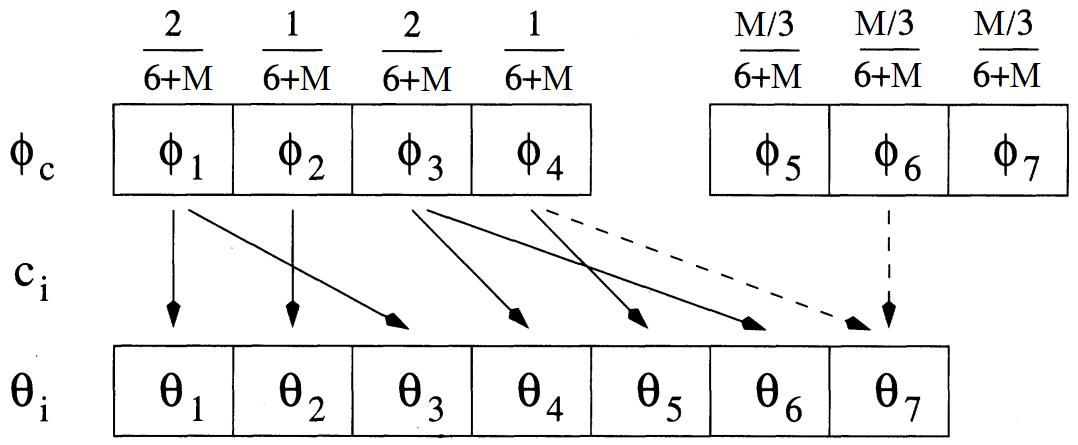
\includegraphics[width=0.9\textwidth]{etc/neal8.png}
    \captionsetup{labelformat=empty}
    \caption{Graphical representation of the variables: the allocations are visualized as arrows linking each $\boldsymbol\theta_i$ with either one of the four old clusters or one of the new components (image taken from \cite{neal})}
    \label{fig:neal8}
\end{figure}

The first step scans all the observations and evaluates each $c_i$.
If it is equal to some other $c_j$, i.e. if the current cluster of observation $i$ is not a singleton, then all auxiliary variables are iid drawn from $G_0$.
If instead the cluster corresponding to $c_i$ is a singleton, then it is linked to one of the auxiliary blocks (i.e. the first one, without loss of generality) while keeping its old unique value $\boldsymbol\phi_{c_i}$ (as shown in the above figure), whereas the other blocks are drawn normally from $G_0$ as before.
Then, $c_i$ is updated according to the following conditional probabilities:
\begin{equation}
	\begin{aligned} \label{neal8prob}
		\PP(c_{i}=c | \boldsymbol c_{-i}, y_{i}, \boldsymbol\phi_{1},\dots,\boldsymbol\phi_{h}) \propto
		\begin{cases}
			\dfrac{n_{-i,c}}{n-1+M}f(y_{i}|\boldsymbol\phi_{c}), & \mbox{for } 1 \leq c \leq k^{-} \\
			\\
			\dfrac{M/m}{n-1+M}f(y_{i}|\boldsymbol\phi_{c}), & \mbox{for } k^{-}+1 < c \leq h,
		\end{cases}
	\end{aligned}
\end{equation}
indicating with $k^{-}$ the number of distinct $c_j$ excluding the current $c_i$ and setting $h=k^{-}+m$.
Again, the probabilities of being placed in an already existing cluster or in a newly created cluster are proportional to the cluster's cardinality (sans observation $i$) and to the total mass, respectively. \\
Once all the $\boldsymbol\phi_c$ that are no longer associated with any observation are discarded, the algorithm proceeds, for each cluster, with the sampling of $\boldsymbol\phi_c$ from the posterior computed with the observations of the specific cluster, similarly to the \verb|Neal2| algorithm.

\section{Blocked Gibbs}
Another Gibbs sampling method that is applicable in the considered DPM model is the one proposed by Ishwaran and James (see \cite{james} section 5), where the prior $P$ is assumed to be a finite dimensional stick-breaking measure, allowing the update of whole blocks of parameters.
A key point of the method is that it does not marginalize over the prior; instead, by grouping more variables together, it samples from their joint distribution conditioned on all other variables.
This sampler needs to draw from the following conditionals:
\begin{align}
	\boldsymbol\phi_1,\dots,\boldsymbol\phi_k &\sim \Lc(\cdot | c_1,\dots,c_n, \boldsymbol{y}) \nonumber \\
	c_1,\dots,c_n &\sim \Lc (\cdot | \boldsymbol\phi_1,\dots,\boldsymbol\phi_k,\boldsymbol{p}, \boldsymbol{y}) \nonumber \\
	\boldsymbol{p} &\sim \Lc (\cdot | c_1,\dots,c_n) \nonumber
\end{align}
The drawing of the unique values can also be handled in the non-conjugate case by applying standard Markov chain Monte Carlo methods. \\
This algorithm is not explored in detail as it has not implemented yet in our library.
For a full explanation, see \cite{james}.

\chapter{Implementation}
As far as code implementation goes, the aforementioned algorithms all share the following structure:
\begin{verbatim}
void step(){
    sample_allocations();
    sample_unique_values();
}

void run(){
    initialize();
    unsigned int iter = 0;
    while(iter < maxiter){
        step();
        if(iter >= burnin){
            save_iteration(iter);
        }
        iter++;
    }
}
\end{verbatim}
In particular, the blocked Gibbs algorithm has an additional phase in \verb|step()|, \verb|sample_weights()|. Moreover, as discussed in chapter \ref{algo}, all the algorithms can be generalized including further Gibbs sampling steps to update the hyperparameters of $G_0$ or the total mass parameter $M$.
Each implemented algorithm will be discussed in detail in its own section.
As for the general structure of an algorithm class, a template approach was chosen, to allow the use of several layers of complexity based on the needs of the user:
\begin{verbatim}
template<template <class> class Hierarchy, class Hypers,
         class Mixture> class Algorithm
\end{verbatim}
That is, \verb|Hierarchy<>|, \verb|Hypers|, and \verb|Mixture| are not actual implemented classes, but rather proxy names for classes which will be received as \emph{parameters} by the algorithm class.
These classes must have a \emph{common interface} in order for them to be passed as parameters, as explained in the following section.
An example with actual class names, as found in the \verb|main.cpp| file, is:
\begin{verbatim}
Neal8<NNIGHierarchy, HypersFixed, SimpleMixture> sampler8;
\end{verbatim}
As a final introductory note, probability distributions and random sampling were handled through the \verb|Stan| library, whilst the popular \verb|Eigen| library was exploited for the creation of the necessary matrix-like objects and the use of matrix-algebraic operations throughout the code.

\section{Auxiliary classes}
First of all, we must briefly describe the auxiliary classes that are used as parameters for the algorithms:
\begin{itemize}
	\item The \verb|Mixture| classes contain all information about the mixing part of the DPM model, namely the total mass parameter and its prior distribution, if any.
	We implemented the \verb|SimpleMixture| class, which represents a fixed total mass parameter without any prior on it, and contains the \verb|totalmass| member as well as a getter and a setter (\verb|get_totalmass()|, \verb|set_totalmass()|).
	\item The \verb|Hypers| classes contain all information about the hyperparameters of the hierarchy, including their values (if fixed) or their prior distributions (if not).
	We implemented the \verb|HypersFixedNNIG| class, which contains the four fixed parameters \verb|mu0|, \verb|lambda|, \verb|alpha0|, and \verb|beta0| of the Normal-NIG hierarchical model, and their respective getters and setters.
	\item The \verb|Hierarchy<Hypers>| classes are template classes themselves and accept any \verb|Hypers| class as template parameter.
	A \verb|Hierarchy<>| class contains a vector \verb|state| which stores the current values of the likelihood parameters, as well as a pointer to a \verb|Hypers| object -- this is why \verb|Hypers| is required as a parameter for \verb|Hierarchy<>|.
	A pointer is chosen instead of an actual object, since multiple \verb|Hierarchy<>| objects will be created and stored by the algorithms; the \verb|state|s of these objects will of course share the same prior, and with a pointer to \verb|Hypers| the updating of the prior will only happen once rather than one time per object.
	A \verb|Hierarchy<>| class also contains functions to:
	\begin{itemize}
		\item evaluate the marginal distribution (provided it is known in closed form) and the log-likelihood in a given set of points, given the current \verb|state|;
		\item compute the posterior parameters with respect to a given set of observations;
		\item generate new values for the \verb|state| both according to its prior and to its posterior distribution;
		\item get and set class members, as with the other classes.
	\end{itemize}
	In particular, we implemented the \verb|HierarchyNNIG| class, which represents the Normal-NIG model described in section \ref{nnig}.
	The \verb|state| holds the values for $\boldsymbol\phi = (\mu,\sigma)$.
\end{itemize}
Any class representing any type of hierarchy or parameters can be built as long as it possesses the above interface, which is required for their use in the implemented algorithms. \\
We will be now first examining the \verb|Neal8| class as an example.

\section{\texttt{Neal8} algorithm}
Relying on the algorithm described in section \ref{neal8}, we proceed to describe our implementation of it.
Aside from the usual getters and setters, as well as constructors, the \verb|Neal8| class contains the following members:
\begin{verbatim}
unsigned int n_aux;
unsigned int maxiter;
unsigned int burnin;
unsigned int num_clusters;
std::mt19937 rng; // random number generating engine
\end{verbatim}
These are the parameters of the method, and are rather self-explanatory.
Their values are initialized either via the constructors or the setters.
If \verb|num_clusters| is not provided, it will be automatically set equal to the number of data points, thus starting the algorithm with one datum per cluster. \\
The data and values containers were implemented as follows:
\begin{verbatim}
std::vector<double> data;
std::vector<unsigned int> allocations;
std::vector<Hierarchy<Hypers>> unique_values;
std::vector<Hierarchy<Hypers>> aux_unique_values;
Mixture mixture;
\end{verbatim}
The algorithm will keep track of the labels representing assignments to clusters via the \verb|allocations| vector.
For instance, if one has \verb|allocations[5] = 2|, it means that datum number 5 is associated to cluster number 2.
Note that indexing for both data and clusters starts at zero, so this actually means that we have the sixth datum being assigned to the third cluster. \\
The containers for the unique values $\boldsymbol\phi$ hold objects of type \verb|Hierarchy<>| because each $\boldsymbol\phi$ is associated to a cluster, which is in fact a small hierarchy that can have its own hyperprior in the general case.
The same reasoning goes for \verb|aux_unique_values|, the $m$ auxiliary blocks, from which the algorithm may draw in order to generate new clusters. \\
As for the members used for running the algorithm:
\begin{verbatim}
void initialize();
void sample_allocations();
void sample_unique_values();
void step(){
    sample_allocations();
    sample_unique_values();
}
void save_iteration(unsigned int iter);
void run();
\end{verbatim}
Aside from \verb|run()|, whose code was shown at the beginning of this section, we shall briefly describe the implementation of these functions:
\begin{itemize}
	\item \verb|initialize()| creates \verb|num_clusters| clusters and randomly assigns each datum to one of them, while making sure that each cluster contains at least one.
	This assignment is done through changing \verb|allocations| components, as explained earlier.
	\item In \verb|sample_allocations()|, a loop is performed over all observations $i=1:n$.
	A vector \verb|card| is first filled, with \verb|card[j]| being the cardinality of cluster $j$.
	The algorithm mandates that \verb|data[i]| be moved to another cluster; thus, if the current cluster is a singleton, its $\boldsymbol\phi$ values are transferred to the first auxiliary block.
	Then, each auxiliary block (except the first one if the above case occurred) generates new $\boldsymbol\phi$ values via the hierarchy's \verb|draw()| function.
	Now a new cluster, that is, new $\boldsymbol\phi$ values, for \verb|data[i]| needs to be drawn.
	A vector \verb|probas| with \verb|n_unique+n_aux| components is filled with the probabilities of each $\boldsymbol\phi$ being extracted, in line with (\ref{neal8prob}).
	Computations involve, among other things, the \verb|card| vector, the likelihood \verb|like()| evaluated in \verb|data[i]|, and the total mass parameter.
	Then, the new value for \verb|allocations[i]| is randomly drawn according to the computed \verb|probas|.
	Finally, four different cases of updating \verb|unique_values| and \verb|card| are handled separately, depending on whether the old cluster was a singleton or not, and whether an auxiliary block or an already existing cluster was chosen as the new cluster for \verb|data[i]|.
	This is done because depending on the case, clusters are either unchanged, increased by one, decreased by one, or moved around.
	\item In \verb|sample_unique_values()|, for each cluster $j$, their $\boldsymbol\phi$ values are updated through the \verb|sample_given_data()| function, which takes as argument the vector \verb|curr_data| of data points which belong to cluster $j$.
	Since we only keep track of clusters via their labels in \verb|allocations|, we do not have a vector of actual data points stored for each cluster.
	Thus we must fill, before the loop on $j$, a matrix \verb|clust_idxs| whose column $k$ contains the index of data points belonging to cluster $k$.
	\verb|clust_idxs| is then used in the $j$ loop to fill \verb|curr_data| with the actual data points of cluster $j$.
	\item \verb|save_iteration| will be examined in the next section.
\end{itemize}

\section{\texttt{Neal2} algorithm}
The structure of the \verb|Neal2| class is similar to the one of \verb|Neal8| described above.
The only relevant differences are the obvious lack of \verb|aux_unique_values| and most of the \verb|sample_allocations()| phase.
As discussed in section \ref{neal2}, this algorithm exploits conjugacy, thus this function requires specifically implemented hierarchies, in which the marginal distribution of the data with respect to $\boldsymbol\theta$ is provided in closed form.
In our case, a Normal-NIG specialization for the \verb|Neal2| template class was implemented.
In \verb|sample_allocations()|, a loop is performed over observations $i$ and the \verb|card| vector is built, just as before.
The \verb|probas| vector of weights for the new allocation value is computed, according to the probabilities (\ref{probasneal2}), by also using the marginal density in \verb|data[i]|, which is known to be a Student's $t$ as mentioned in section \ref{nnig}.
After the new \verb|allocations[i]| is drawn according to \verb|probas|, four cases are handled separately as before, depending on whether the old cluster was a singleton and whether \verb|data[i]| is assigned to a new cluster.
Indeed, in such a case, a new $\boldsymbol\phi$ value for it must be generated, and this must be handled differently by the code if an old singleton cluster was just destroyed (as the new cluster must take its former place).

\part{Applications}

\chapter{Applications}
These algorithms can also be used for two useful practical purposes: \emph{cluster estimation} and \emph{density estimation}.
Both processes, however, require the whole chain to be saved, that is, at each iteration the current values of states and allocations must be stored in some data structure.
For this purpose, we used the Protocol Buffers library, which needs a short introduction. \\
Protocol Buffers, or \verb|protobuf| for short, was developed by Google and allows automatic generation of data-storing C++ classes by defining a class skeleton in a \verb|.proto| file.
This also allows easy interfacing with other programming languages such as R and Python. \\
We built our template as follows:
\begin{verbatim}
message UniqueValues {
    repeated double params = 1;
}
message IterationOutput {
    repeated int32 allocations = 1;
    repeated UniqueValues phi = 2;
}
message ChainOutput {
    repeated IterationOutput state = 1;
}
\end{verbatim}
Here \verb|message| and \verb|repeated| are the \verb|protobuf| equivalent of classes and vectors respectively, while the numbers 1 and 2 just act as identifiers for the fields in the messages.
After generating the corresponding C++ classes via the \verb|protoc| compiler, we were able to add the following members to the \verb|Neal8| and \verb|Neal2| classes:
\begin{verbatim}
ChainOutput chain;
IterationOutput best_clust;
std::pair< std::vector<double>, Eigen::VectorXd > density;
\end{verbatim}
For each iteration after the burn-in phase, the \verb|save_iteration()| function saves all state values of the current iteration into the \verb|chain| pseudo-vector in the appropriate structure.
On the other hand, \verb|best_clust| represents the state of a single iteration, and it is the object where the result of the clustering analysis will be saved.
The \verb|density| object shares a similar purpose for the density estimation part, albeit not actually generated via \verb|protobuf|.
It will be filled with a grid of points in which the density will be evaluated, and the evaluations of the density themselves. \\
We will be explaining in thorough detail these two useful applications in the next lines.

\section{Cluster estimation}
Suppose we wish to estimate the real clustering of the data, assuming the DPM model holds true.
A first rough estimate is the \emph{final clustering}, that is, the state values corresponding to the last iteration of the algorithm.
This estimate does not require an appropriate function to be implemented, since the state values are already available in \verb|allocations| and \verb|unique_values| after the algorithm is \verb|run()|.
However, due to the oscillating behavior of the clusters (as we shall see later on), the last clustering may not be the optimal one.
Instead, we chose to implement a \emph{least square} estimate in the following function:
\begin{verbatim}
unsigned int cluster_estimate();
\end{verbatim}
This function exploits the \verb|chain| pseudo-vector, in which states of all iterations of the algorithm were saved via \verb|save_iteration()| (of course, only after the burn-in phase) and the \verb|protobuf| library.
This function loops over all \verb|IterationOutput| objects in \verb|chain|, finds the iteration at which the best clustering occurred, saves the whole object into the \verb|best_clust| class member, and returns the iteration number of this best clustering.
As briefly touched upon earlier, the best clustering is found via the minimization of the squared posterior \emph{Binder's loss function}.
An equivalent approach (see \cite{beep} lecture on BNP clustering) is computing the so-called \emph{dissimilarity matrix} for each iteration, computing its sample mean over all iterations, and finding the iteration that is the closest to the mean with respect to the \emph{Frobenius norm}. 
More specifically, for each iteration $k$, the dissimilarity matrix $D^{(k)}$ is a symmetric, binary $n$-by-$n$ matrix (where $n$ is the number of available observations) whose entries $D^{(k)}_{ij}$ are $1$ if datum $i$ and $j$ are placed in the same cluster at iteration $k$ and $0$ otherwise.
After each $D^{(k)}$ and the sample mean $\bar{D} = \frac{1}{K} \sum_k D^{(k)}$ are computed, where $K$ is the number of iterations (not counting the ones in the burn-in phase), the best clustering $\hat{k}$ is found by minimizing the Frobenius norm of the difference with $\bar{D}$:
$$
\hat{k} = \argmin_k \left\lVert D^{(k)} - \bar D \right\rVert_F^2 = \argmin_k \sum_{i,j} \left( D^{(k)}_{ij} - \bar{D}_{ij} \right)^2.
$$
By virtue of the involved matrices being symmetric, the latter summation can be computed over all $i<j$ instead of all $i,j$ for efficiency. \\
The convergence in mean of the algorithm grants the correctness of this least square estimate, at it is the closest available approximation to the mean dissimilarity matrix.

\section{Density estimation} \label{dens-estim}
One other important application of clustering algorithms is the estimation of the density according to which the data points are distributed.
This is done differently in both the \verb|Neal2| and \verb|Neal8| algorithms, as the former can exploit the conjugacy of the hierarchical model.
In either case, the following function was implemented:
\begin{verbatim}
void eval_density(const std::vector<double> grid);
\end{verbatim}
It accepts a grid of points in which the density will be evaluated.
This grid is stored in the \verb|density| member object, as well as the computed evaluations themselves in form of a vector from the \verb|Eigen| library.
Just like for the cluster estimate, the computation will access all iterations stored in the \verb|chain| pseudo-vector.
In both \verb|Neal8| and \verb|Neal2|, a loop is performed over the iterations $k$.
Suppose this iterations has $J$ clusters, that is, $j=0:J-1$.
The \verb|card| vector is once again computed, where $\texttt{card[j]} = n^{(k)}_j$ is the cardinality of cluster $j$.
Then, for each point $x$ in \verb|grid|, we compute the local estimate of the density, that is, only taking iteration $k$ into account:
\begin{equation}\label{localdens}
	\begin{aligned}
	\hat f^{(k)}(x) \ = \ \sum_j \frac{n^{(k)}_j}{M+n} f\left(x | \boldsymbol{\phi}^{(k)}_j\right) \ + \ \frac{M}{M+n} m(x)
	\end{aligned}
\end{equation}
That is, the local estimate is a weighted mean of the likelihood given the unique values $\boldsymbol{\phi}^{(k)}_j$ of cluster $j$ and the marginal distribution $m(x)$, taken from the appropriate function in the \verb|Hierarchy<>| class.
The weights of the clusters are proportional to their size $n^{(k)}_j$, while the ``virtual'' cluster of the marginal counts as having size $M$, the total mass parameter ($n$ is the total number of observations, as per usual).
The marginal distribution is only known under the conjugacy assumption in the \verb|Neal2| algorithm.
In particular, for a Normal-NIG model $m(x)$ is a Student's $t$ as explained in section \ref{nnig}.
In the \verb|Neal8| algorithm, $m(x)$ is not available in closed form, and thus it is replaced in the above formula by the following approximation:
\begin{equation}\label{margneal8}
	\begin{aligned}
		\hat m(x) = \frac{1}{m} \sum_{h=0}^{m-1}  f\left(x | \boldsymbol{\phi}_h\right)
	\end{aligned}
\end{equation}
where we use $m$ unique values, that is, one for each of the $m = \verb|n_aux|$ auxiliary blocks of the algorithm, drawn from the base measure: $\boldsymbol{\phi}_{h} \overset{\text{iid}}{\sim} G_0, \ h=0:m-1$. \\
Finally, the \emph{empirical density} is computed as the mean over all $K$ iterations:
$$
\hat f(x) = \frac{1}{K} \sum_k \hat f^{(k)}(x)
$$
and saved into the \verb|density| object.
Again, this estimate approaches the true posterior density of the data thanks to the convergence in mean of the chain.

\section{Saving estimates to files}
We also implemented the following functions in each \verb|Algorithm| class, which save data from the class into text files in order to ease exportation to other programs or computers:
\begin{verbatim}
const void write_final_clustering_to_file(
           std::string filename = "final_clust.csv");
const void write_best_clustering_to_file(
           std::string filename = "best_clust.csv");
const void write_chain_to_file(
           std::string filename = "chain.csv");
const void write_density_to_file(
           std::string filename = "density.csv");
\end{verbatim}
They can be called as need be from the \verb|main.cpp| file.
If a file name is not provided, the above default names will be used.
The former two create a \verb|.csv| file with the columns being, in order, data index, data value, allocation, unique values (one per column).
\verb|write_chain_to_file()| has the same columns as the previous functions, but adds one more column containing the iteration number (starting from $0$) as the first one.
Finally, \verb|write_density_to_file()| has values of $x$ in the first column and the corresponding $\hat f(x)$ in the second one.

\chapter{Results}
Our clustering analysis was conducted on $n=100$ observations, the former 50 of which were iid sampled from a $\Nc(4,1)$ and the latter from a $\Nc(7,1)$, which were saved in the \verb|data.csv| file.
We chose the prior parameters for the Normal-NIG model (\ref{nnig}) as follows: $\mu_0 = 5, \lambda_0 = 1, \alpha_0 = 2, \beta_0 = 2$.
The \verb|Neal8| algorithm with $m=3$ auxiliary blocks was run for 20000 iterations, and the first 5000 were discarded as burn-in, for a total of $K=15000$ valid iterations.
We will keep these parameters values fixed unless explicitly stated. \\
The following test data were all saved to \verb|.csv| files and used for the realization of plots with the \verb|ggplot2| R package.
All scripts and data sheets are available in the GitHub repository of our library.

\section{Oscillations}
After running the algorithm as described above with total mass $M=0.25$, we find that the obtained best clusterings (again, in the lest square sense) and local density estimates are highly fluctuating over the iterations of the algorithm:
\begin{figure}[h]
	\centering
	\begin{minipage}{0.5\textwidth}
		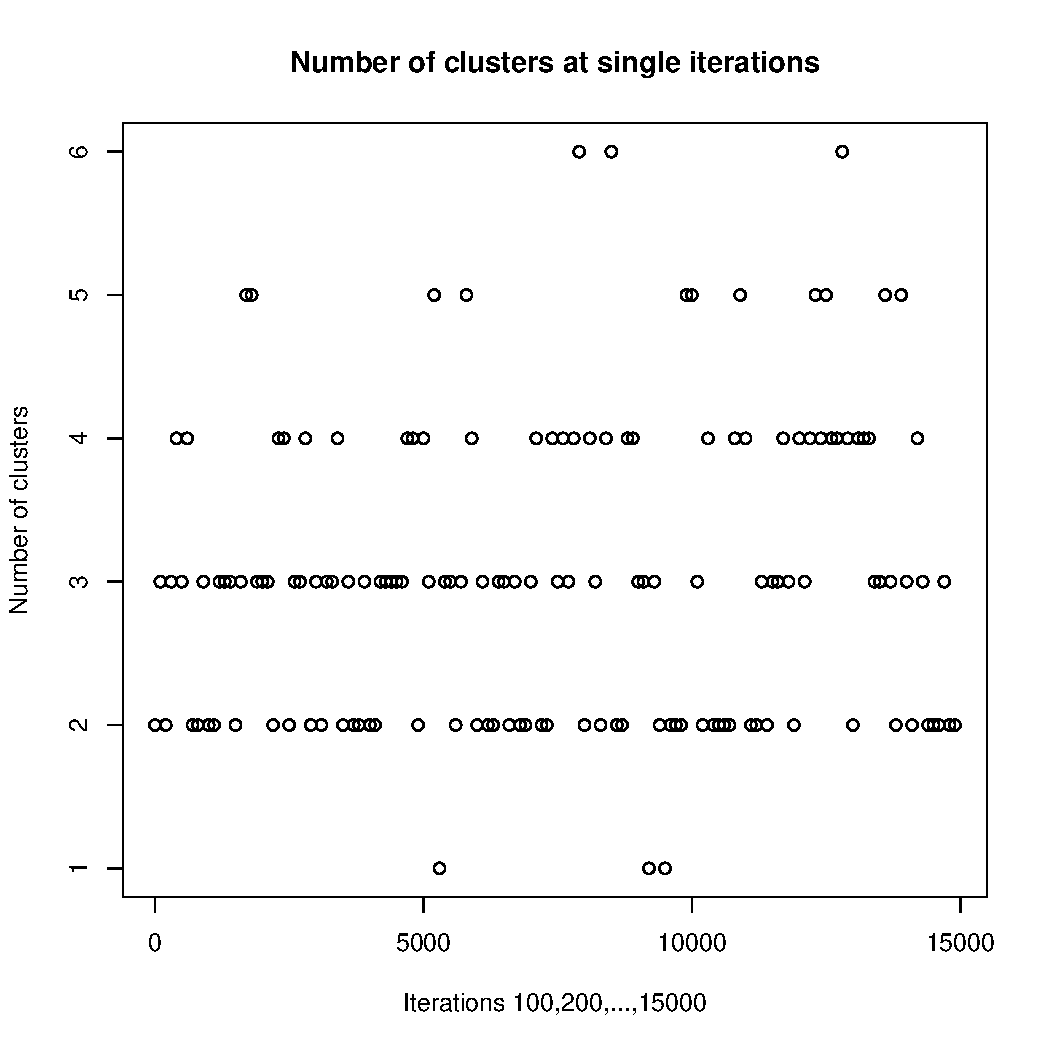
\includegraphics[scale=0.35]{etc/cardinalities_thinned.pdf}
	\end{minipage}%
	\begin{minipage}{0.5\textwidth}
		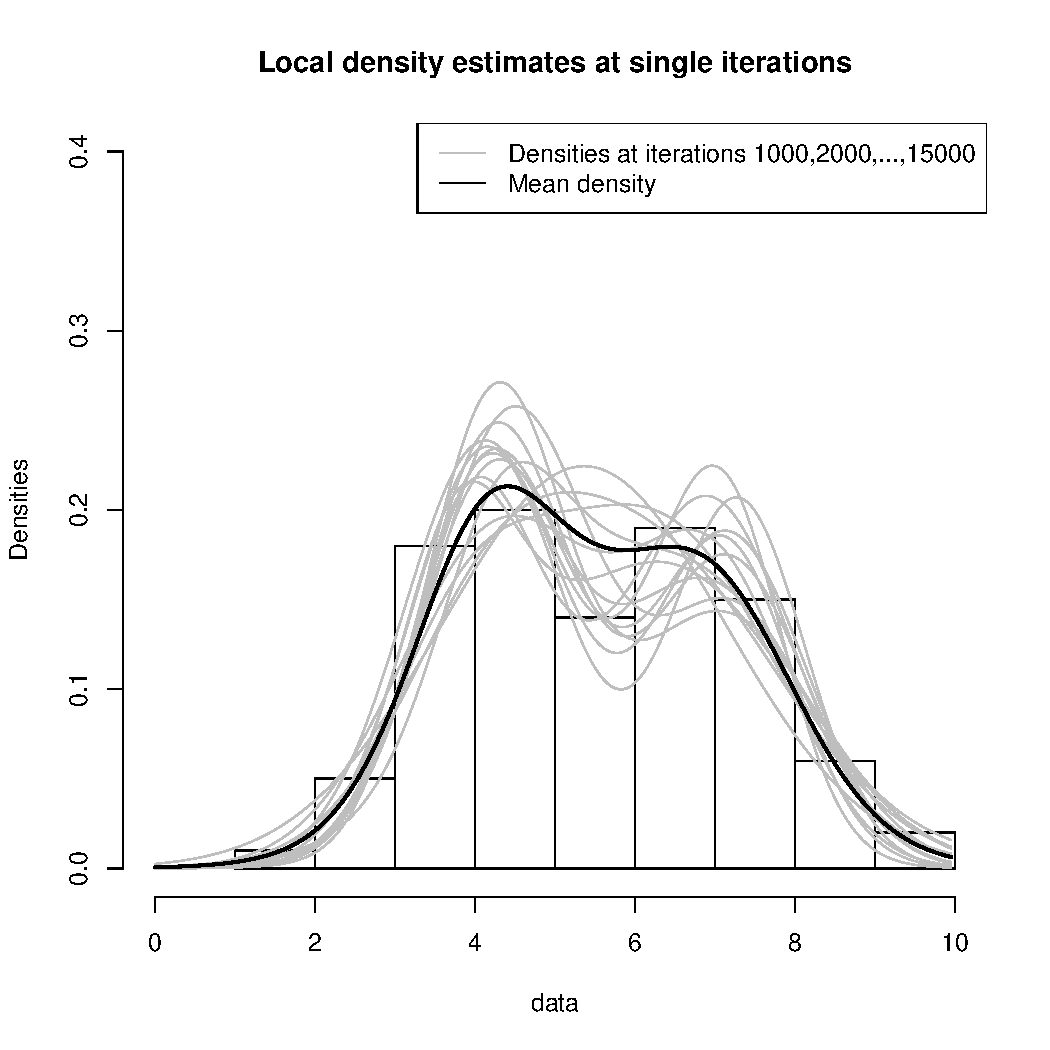
\includegraphics[scale=0.35]{etc/densities_iters.pdf}
	\end{minipage}
\end{figure}

In both plots, a thinning of one iteration every 100 and every 2500, respectively, was performed for better readability of the plot.
In the right side plot, the local densities are compared with the histogram of the data as well as the final estimate provided by the mean density.
We can see that the number of clusters at all iterations varies significantly between 1 and 6, even in the last thousands of iterations, and the same behavior applies to the local density estimates. 
This is further confirmation of the fact that the single iterations themselves do not converge.
Instead, as previously discussed, the convergence is in the \emph{mean}, both for the density estimate and for the average dissimilarity matrix which we use to find the best clustering.

\section{Total mass}
Let us now examine the role of the total mass parameter, $M$.
We ran the algorithm with several values for $M$ whilst keeping the other parameters unchanged from the ones indicated at the beginning of the section.
For each $M$, we saved the number of clusters of the best clustering produced by the algorithm, and plotted it against the corresponding $M$:

\begin{figure}[h]
	\centering
	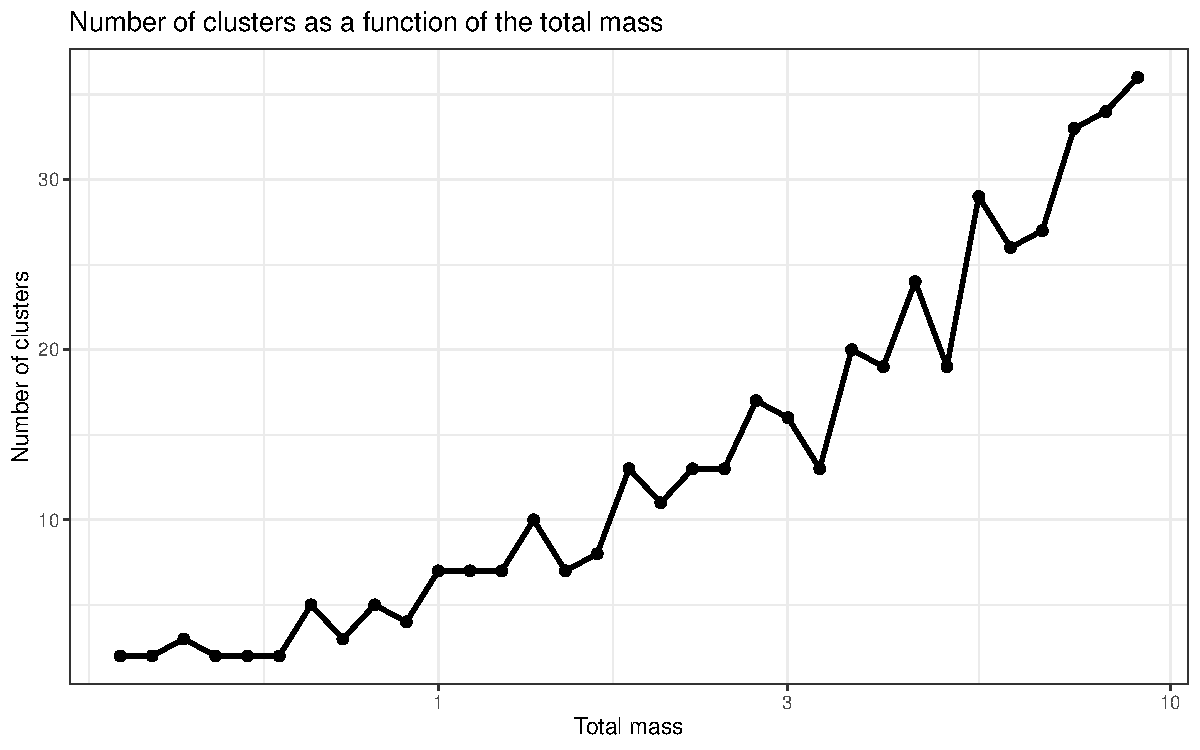
\includegraphics[scale=0.6]{etc/num_clust_M.pdf}
\end{figure}

Note that the values for $M$ were chosen so as to be evenly spaced in log-scale, thus the abscissa is in log-scale as well.
We can note that the clusters are increasing with the total mass.
This is consistent with the fact that the probability of creating a new cluster is proportional to $M$, as seen in (\ref{neal8prob}). \\
Moreover, the density estimates for some of the values of $M$ (again, compared with the histogram of the data) are as follows:

\clearpage

\begin{figure}[h]
	\centering
	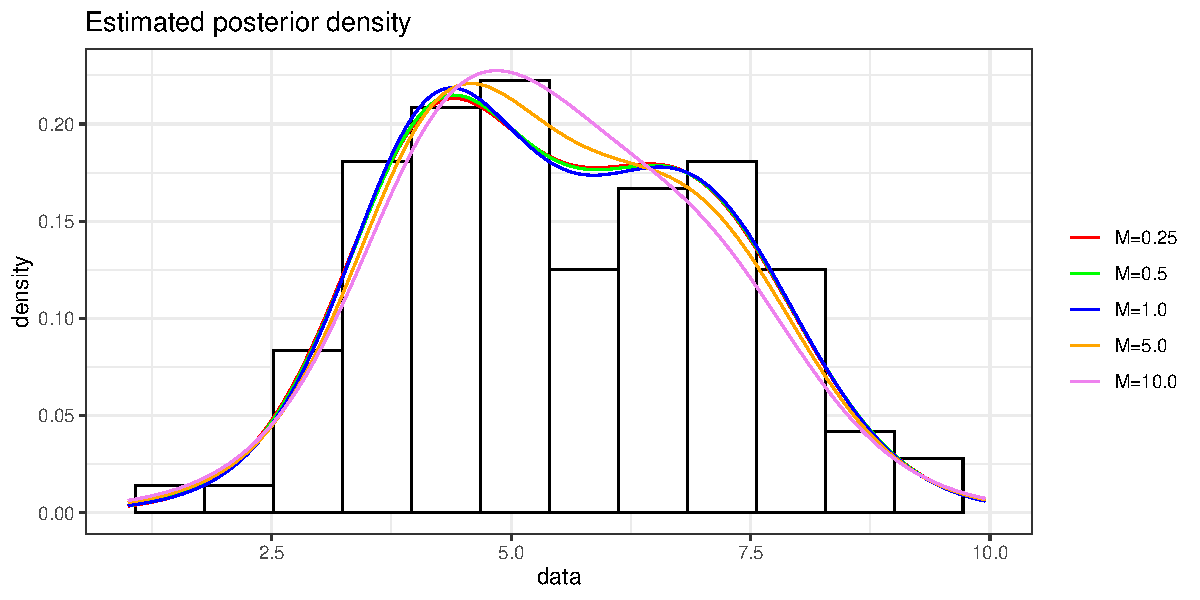
\includegraphics[scale=0.6]{etc/dens_withMm3.pdf}
\end{figure}


In our case, lower values for the total mass account better for the distribution of the data points, with the modes being near the real expected values of the two normal distributions, 4 and 7.
On the other hand, higher values tend to clump together all 100 observations as though they were extracted from a single distribution.
As we can see, the total mass $M$ acts as smoothing parameter and, given its strong influence on the number of mixture components, it is a prime candidate for a prior distribution being put onto it.



\section{Auxiliary blocks}
We shall now try and change the number of auxiliary blocks $m$, and check how this impacts the density estimation.
For this test, a large total mass $M=10$ was chosen; the reason being that a small $M$ would not allow significant differences as $m$ changes.
Indeed, $m$ directly influences only the estimate (\ref{margneal8}) of the marginal distribution, that has a weight of $\frac{M}{M+n}$ (as seen in (\ref{localdens})), which is negligible if $M$ is small.
Therefore, $M=10$ was picked, and the result was the following:


\begin{figure}[h]
	\centering
	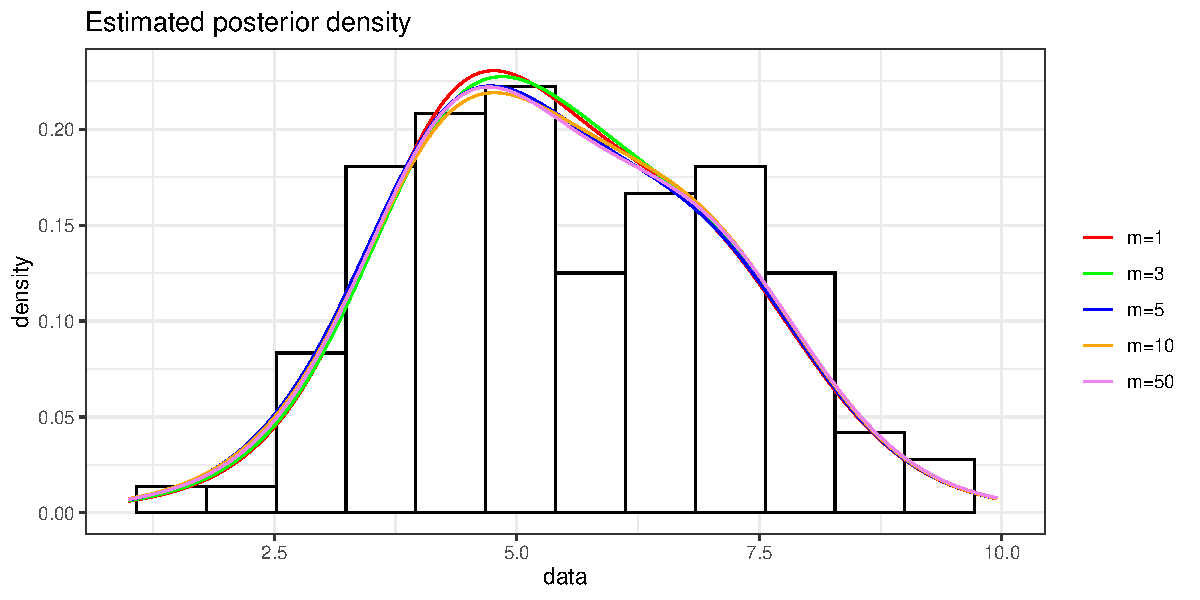
\includegraphics[scale=0.6]{etc/dens_withmM10.pdf}
\end{figure}

Note that a larger $m$ gives a better estimate of the marginal, because the sample mean is computed over a larger number of terms and the algorithm approximates the behavior of the algorithm \verb|Neal2|.



\section{Density components}
We now wish to visualize how the local density is computed at a given sample iteration.
Let us run again the \verb|Neal8| algorithm with both $M=0.25$ and $m=3$ fixed, and then use the \verb|cluster_estimate()| function to extract the best clustering for the data.
We find that it is at iteration 2490, which gives 2 clusters.
As shown in \ref{localdens}, each of these clusters has its own density estimate, which we refer to as \emph{component}, and a weight attached to it proportional to its cardinality.
The weighted sum of these components gives the ``full'' local estimate of the density for that iteration.
This plot shows both the \emph{weighted} components and their sum:
\begin{figure}[h]
	\centering
	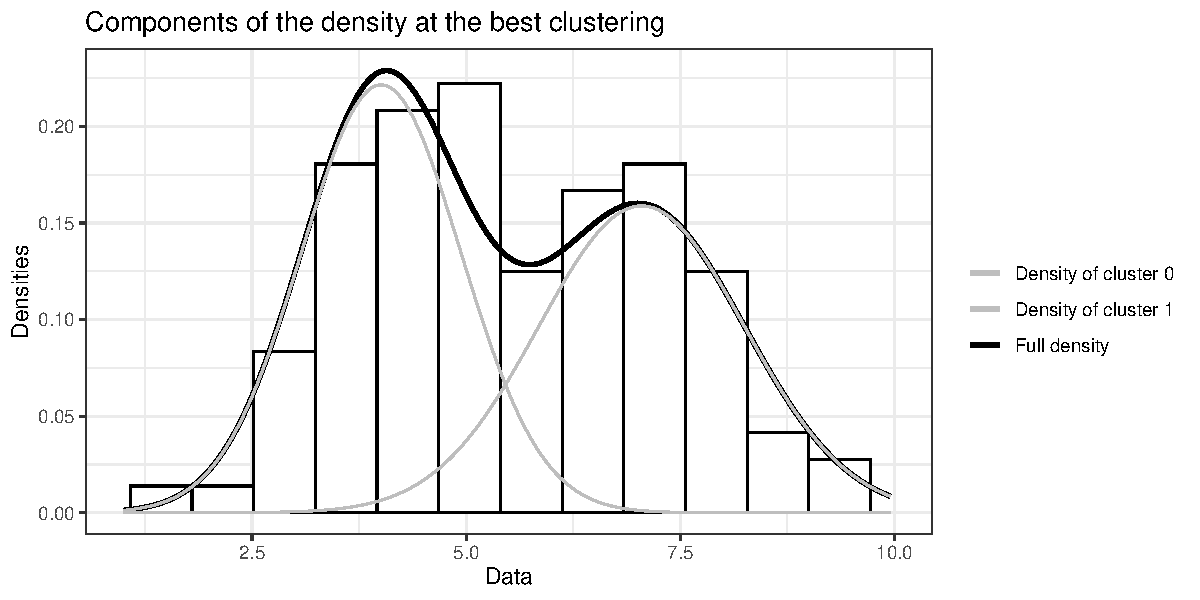
\includegraphics[scale=0.7]{etc/componentsM025m3_best.pdf}
\end{figure}

In this case the weights turn out to be approximately equal (0.52 and 0.48 respectively).
Again, the two components are concentrated around the true means (4 and 7) of the likelihoods of the data points, as expected. \\
In other cases, the best clustering may produce more than 2 clusters.
One such example is given by the best clustering of \verb|Neal8| run with $M=1$ (and $m=3$ as before), found at iteration 6611.
Although there are 7 clusters, all weights bar the first two are insignificant, making the corresponding components have almost zero impact in the weighted sum of the local estimate:

\clearpage

\begin{figure}[h]
	\centering
	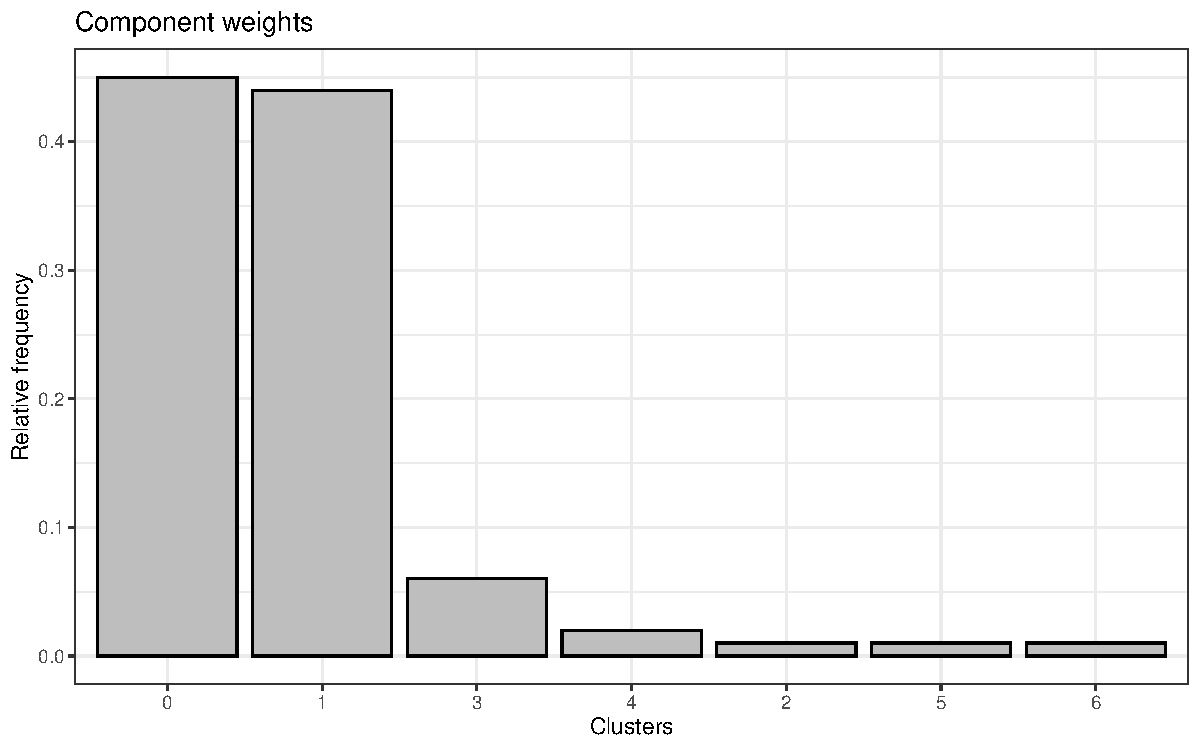
\includegraphics[scale=0.5]{etc/barplotM1m3.pdf}
\end{figure}



\section{\texttt{Neal2} vs \texttt{Neal8}}
Finally, we ran the \verb|Neal2| algorithm with the same parameters as \verb|Neal8| (indicated at the beginning of the section) as well as $M=10$ for both.
Again, a rather large total mass was chosen in order to better highlight the difference in the marginal estimate.
In fact, in the \verb|Neal2| case, since the marginal distribution is known in closed form, the estimate is more accurate:

\begin{figure}[h]
	\centering
	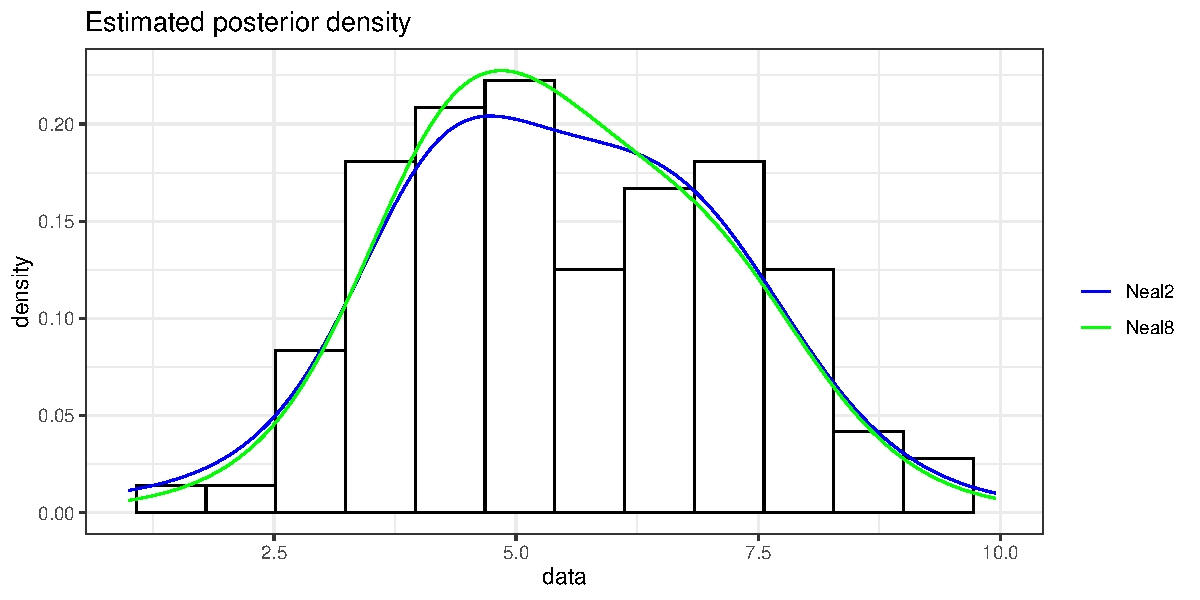
\includegraphics[scale=0.7]{etc/neal2_M10.pdf}
\end{figure}

\chapter{Extensions}
The \verb|bnplib| library has several possible extensions:
\begin{itemize}
	\item New types of \verb|Hypers| classes can be implemented, for example ones containing hyper-priors for some of the parameters if the model.
	The algorithm must be modified accordingly, for instance by adding extra steps (which are skipped if the hyperparameters are fixed).
	Changes depend on the type of parameter for which a prior is used; for example, a prior on the total mass parameter involves different steps than a prior on the parameters of the base measure.
	For a general outline of the necessary changes, see \cite{neal} section 7.
	\item Hierarchies other than the Normal-NIG can be created.
	This is enough to run \verb|Neal8| and \verb|Neal2| by passing the class name as parameter, provided that the \verb|Hierarchy| class has the appropriate interface.
	\item Interfaces with both R and Python can be easily implemented, thanks to the data structures provided by \verb|protobuf| and the already-available libraries \verb|Rcpp| and \verb|pybind| respectively.
	\item Algorithms can be re-adapted for the use of other mixture models, such as the Pitman-Yor process.
	\item Conjugacy-dependent algorithms such as \verb|Neal2| can be re-adapted to account for non-conjugacy, for example by using an Hamiltonian Monte Carlo sampler.
	\item Finally, a \emph{full generalization} of the library might be possible.
	That is, given the distributions of the likelihood, hyperparameters, etc, one might want an algorithm that works for the chosen specific model without needing and explicit implementation for it.
	This means, among other things, that one has to handle non-conjugacy for the general case.
	The main issue is that Stan distribution functions do not accept vectors of parameter values as arguments; thus, the updated values for distributions must be explicitly enumerated and given as arguments one by one to the Stan function.
	This requires to know in advance the number of parameters for all such distributions, which is impossible in the general case.
	Some advanced C++ techniques may be used to circumvent this hindrance, such as argument unpackers that transform a vector into a list of function arguments, and variadic templates, which are templates that accept any number of arguments.
	Theoretically, the latter would also allow the use of priors on the parameters of the hyper-prior itself, and so on, adding layers of uncertainty ad libitum.
	Although it is a hard task, we do think it is possible to achieve with reasonable effort.
\end{itemize}


\begin{thebibliography}{9}
	\bibitem{book} P. Muller, F. A. Quintana, \textit{Bayesian Nonparametric Data Analysis}
	
	\bibitem{neal} R. M. Neal (2000), \textit{Markov Chain Sampling Methods for Dirichlet Process Mixture Models}
	
	\bibitem{james} H. Ishwaran, L. F. James (2001), \textit{Gibbs Sampling Methods for Stick-Breaking Priors}
	
	\bibitem{integral} K. P. Murphy (2007), \textit{Conjugate Bayesian analysis of the Gaussian distribution}
	
	\bibitem{stan} Stan documentation: \url{http://mc-stan.org/math}. \\
	Code found at \url{https://github.com/stan-dev/math} (version 3.0.0 was used) and it also includes other needed libraries: Boost, Eigen, SUNDIALS, Intel TBB
	
	\bibitem{eigen} Eigen documentation: \url{https://eigen.tuxfamily.org/dox}. \\
	Code is included in the Stan package (version 3.3.3 is used there)
	
	\bibitem{proto} Protocol Buffers Tutorial for C++: \url{https://developers.google.com/protocol-buffers/docs/cpptutorial}. \\
	Code found at \url{https://github.com/protocolbuffers/protobuf} (version 3.11.0 was used)
	
	\bibitem{tutors} Codes of Mario Beraha and Riccardo Corradin for similar projects, found at \url{https://github.com/mberaha/partial_exchangeability} and \url{https://github.com/rcorradin/BNPmix} respectively
	
	\bibitem{beep} Course material for Bayesian Statistics: \url{https://beep.metid.polimi.it/web/2019-20-bayesian-statistics-alessandra-guglielmi-/}
\end{thebibliography}

\end{document}
